
%% bare_conf.tex
%% V1.4b
%% 2015/08/26
%% by Michael Shell
%% See:
%% http://www.michaelshell.org/
%% for current contact information.
%%
%% This is a skeleton file demonstrating the use of IEEEtran.cls
%% (requires IEEEtran.cls version 1.8b or later) with an IEEE
%% conference paper.
%%
%% Support sites:
%% http://www.michaelshell.org/tex/ieeetran/
%% http://www.ctan.org/pkg/ieeetran
%% and
%% http://www.ieee.org/

%%*************************************************************************
%% Legal Notice:
%% This code is offered as-is without any warranty either expressed or
%% implied; without even the implied warranty of MERCHANTABILITY or
%% FITNESS FOR A PARTICULAR PURPOSE! 
%% User assumes all risk.
%% In no event shall the IEEE or any contributor to this code be liable for
%% any damages or losses, including, but not limited to, incidental,
%% consequential, or any other damages, resulting from the use or misuse
%% of any information contained here.
%%
%% All comments are the opinions of their respective authors and are not
%% necessarily endorsed by the IEEE.
%%
%% This work is distributed under the LaTeX Project Public License (LPPL)
%% ( http://www.latex-project.org/ ) version 1.3, and may be freely used,
%% distributed and modified. A copy of the LPPL, version 1.3, is included
%% in the base LaTeX documentation of all distributions of LaTeX released
%% 2003/12/01 or later.
%% Retain all contribution notices and credits.
%% ** Modified files should be clearly indicated as such, including  **
%% ** renaming them and changing author support contact information. **
%%*************************************************************************


% *** Authors should verify (and, if needed, correct) their LaTeX system  ***
% *** with the testflow diagnostic prior to trusting their LaTeX platform ***
% *** with production work. The IEEE's font choices and paper sizes can   ***
% *** trigger bugs that do not appear when using other class files.       ***                          ***
% The testflow support page is at:
% http://www.michaelshell.org/tex/testflow/



\documentclass[conference]{IEEEtran}
% Some Computer Society conferences also require the compsoc mode option,
% but others use the standard conference format.
%
% If IEEEtran.cls has not been installed into the LaTeX system files,
% manually specify the path to it like:
% \documentclass[conference]{../sty/IEEEtran}





% Some very useful LaTeX packages include:
% (uncomment the ones you want to load)


% *** MISC UTILITY PACKAGES ***
%
%\usepackage{ifpdf}
% Heiko Oberdiek's ifpdf.sty is very useful if you need conditional
% compilation based on whether the output is pdf or dvi.
% usage:
% \ifpdf
%   % pdf code
% \else
%   % dvi code
% \fi
% The latest version of ifpdf.sty can be obtained from:
% http://www.ctan.org/pkg/ifpdf
% Also, note that IEEEtran.cls V1.7 and later provides a builtin
% \ifCLASSINFOpdf conditional that works the same way.
% When switching from latex to pdflatex and vice-versa, the compiler may
% have to be run twice to clear warning/error messages.






% *** CITATION PACKAGES ***
%
%\usepackage{cite}
% cite.sty was written by Donald Arseneau
% V1.6 and later of IEEEtran pre-defines the format of the cite.sty package
% \cite{} output to follow that of the IEEE. Loading the cite package will
% result in citation numbers being automatically sorted and properly
% "compressed/ranged". e.g., [1], [9], [2], [7], [5], [6] without using
% cite.sty will become [1], [2], [5]--[7], [9] using cite.sty. cite.sty's
% \cite will automatically add leading space, if needed. Use cite.sty's
% noadjust option (cite.sty V3.8 and later) if you want to turn this off
% such as if a citation ever needs to be enclosed in parenthesis.
% cite.sty is already installed on most LaTeX systems. Be sure and use
% version 5.0 (2009-03-20) and later if using hyperref.sty.
% The latest version can be obtained at:
% http://www.ctan.org/pkg/cite
% The documentation is contained in the cite.sty file itself.






% *** GRAPHICS RELATED PACKAGES ***
%
\ifCLASSINFOpdf
  % \usepackage[pdftex]{graphicx}
  % declare the path(s) where your graphic files are
  % \graphicspath{{../pdf/}{../jpeg/}}
  % and their extensions so you won't have to specify these with
  % every instance of \includegraphics
  % \DeclareGraphicsExtensions{.pdf,.jpeg,.png}
\else
  % or other class option (dvipsone, dvipdf, if not using dvips). graphicx
  % will default to the driver specified in the system graphics.cfg if no
  % driver is specified.
  % \usepackage[dvips]{graphicx}
  % declare the path(s) where your graphic files are
  % \graphicspath{{../eps/}}
  % and their extensions so you won't have to specify these with
  % every instance of \includegraphics
  % \DeclareGraphicsExtensions{.eps}
\fi
% graphicx was written by David Carlisle and Sebastian Rahtz. It is
% required if you want graphics, photos, etc. graphicx.sty is already
% installed on most LaTeX systems. The latest version and documentation
% can be obtained at: 
% http://www.ctan.org/pkg/graphicx
% Another good source of documentation is "Using Imported Graphics in
% LaTeX2e" by Keith Reckdahl which can be found at:
% http://www.ctan.org/pkg/epslatex
%
% latex, and pdflatex in dvi mode, support graphics in encapsulated
% postscript (.eps) format. pdflatex in pdf mode supports graphics
% in .pdf, .jpeg, .png and .mps (metapost) formats. Users should ensure
% that all non-photo figures use a vector format (.eps, .pdf, .mps) and
% not a bitmapped formats (.jpeg, .png). The IEEE frowns on bitmapped formats
% which can result in "jaggedy"/blurry rendering of lines and letters as
% well as large increases in file sizes.
%
% You can find documentation about the pdfTeX application at:
% http://www.tug.org/applications/pdftex





% *** MATH PACKAGES ***
%
%\usepackage{amsmath}
% A popular package from the American Mathematical Society that provides
% many useful and powerful commands for dealing with mathematics.
%
% Note that the amsmath package sets \interdisplaylinepenalty to 10000
% thus preventing page breaks from occurring within multiline equations. Use:
%\interdisplaylinepenalty=2500
% after loading amsmath to restore such page breaks as IEEEtran.cls normally
% does. amsmath.sty is already installed on most LaTeX systems. The latest
% version and documentation can be obtained at:
% http://www.ctan.org/pkg/amsmath





% *** SPECIALIZED LIST PACKAGES ***
%
%\usepackage{algorithmic}
% algorithmic.sty was written by Peter Williams and Rogerio Brito.
% This package provides an algorithmic environment fo describing algorithms.
% You can use the algorithmic environment in-text or within a figure
% environment to provide for a floating algorithm. Do NOT use the algorithm
% floating environment provided by algorithm.sty (by the same authors) or
% algorithm2e.sty (by Christophe Fiorio) as the IEEE does not use dedicated
% algorithm float types and packages that provide these will not provide
% correct IEEE style captions. The latest version and documentation of
% algorithmic.sty can be obtained at:
% http://www.ctan.org/pkg/algorithms
% Also of interest may be the (relatively newer and more customizable)
% algorithmicx.sty package by Szasz Janos:
% http://www.ctan.org/pkg/algorithmicx




% *** ALIGNMENT PACKAGES ***
%
%\usepackage{array}
% Frank Mittelbach's and David Carlisle's array.sty patches and improves
% the standard LaTeX2e array and tabular environments to provide better
% appearance and additional user controls. As the default LaTeX2e table
% generation code is lacking to the point of almost being broken with
% respect to the quality of the end results, all users are strongly
% advised to use an enhanced (at the very least that provided by array.sty)
% set of table tools. array.sty is already installed on most systems. The
% latest version and documentation can be obtained at:
% http://www.ctan.org/pkg/array


% IEEEtran contains the IEEEeqnarray family of commands that can be used to
% generate multiline equations as well as matrices, tables, etc., of high
% quality.




% *** SUBFIGURE PACKAGES ***
%\ifCLASSOPTIONcompsoc
%  \usepackage[caption=false,font=normalsize,labelfont=sf,textfont=sf]{subfig}
%\else
%  \usepackage[caption=false,font=footnotesize]{subfig}
%\fi
% subfig.sty, written by Steven Douglas Cochran, is the modern replacement
% for subfigure.sty, the latter of which is no longer maintained and is
% incompatible with some LaTeX packages including fixltx2e. However,
% subfig.sty requires and automatically loads Axel Sommerfeldt's caption.sty
% which will override IEEEtran.cls' handling of captions and this will result
% in non-IEEE style figure/table captions. To prevent this problem, be sure
% and invoke subfig.sty's "caption=false" package option (available since
% subfig.sty version 1.3, 2005/06/28) as this is will preserve IEEEtran.cls
% handling of captions.
% Note that the Computer Society format requires a larger sans serif font
% than the serif footnote size font used in traditional IEEE formatting
% and thus the need to invoke different subfig.sty package options depending
% on whether compsoc mode has been enabled.
%
% The latest version and documentation of subfig.sty can be obtained at:
% http://www.ctan.org/pkg/subfig




% *** FLOAT PACKAGES ***
%
%\usepackage{fixltx2e}
% fixltx2e, the successor to the earlier fix2col.sty, was written by
% Frank Mittelbach and David Carlisle. This package corrects a few problems
% in the LaTeX2e kernel, the most notable of which is that in current
% LaTeX2e releases, the ordering of single and double column floats is not
% guaranteed to be preserved. Thus, an unpatched LaTeX2e can allow a
% single column figure to be placed prior to an earlier double column
% figure.
% Be aware that LaTeX2e kernels dated 2015 and later have fixltx2e.sty's
% corrections already built into the system in which case a warning will
% be issued if an attempt is made to load fixltx2e.sty as it is no longer
% needed.
% The latest version and documentation can be found at:
% http://www.ctan.org/pkg/fixltx2e


%\usepackage{stfloats}
% stfloats.sty was written by Sigitas Tolusis. This package gives LaTeX2e
% the ability to do double column floats at the bottom of the page as well
% as the top. (e.g., "\begin{figure*}[!b]" is not normally possible in
% LaTeX2e). It also provides a command:
%\fnbelowfloat
% to enable the placement of footnotes below bottom floats (the standard
% LaTeX2e kernel puts them above bottom floats). This is an invasive package
% which rewrites many portions of the LaTeX2e float routines. It may not work
% with other packages that modify the LaTeX2e float routines. The latest
% version and documentation can be obtained at:
% http://www.ctan.org/pkg/stfloats
% Do not use the stfloats baselinefloat ability as the IEEE does not allow
% \baselineskip to stretch. Authors submitting work to the IEEE should note
% that the IEEE rarely uses double column equations and that authors should try
% to avoid such use. Do not be tempted to use the cuted.sty or midfloat.sty
% packages (also by Sigitas Tolusis) as the IEEE does not format its papers in
% such ways.
% Do not attempt to use stfloats with fixltx2e as they are incompatible.
% Instead, use Morten Hogholm'a dblfloatfix which combines the features
% of both fixltx2e and stfloats:
%
% \usepackage{dblfloatfix}
% The latest version can be found at:
% http://www.ctan.org/pkg/dblfloatfix




% *** PDF, URL AND HYPERLINK PACKAGES ***
%
%\usepackage{url}
% url.sty was written by Donald Arseneau. It provides better support for
% handling and breaking URLs. url.sty is already installed on most LaTeX
% systems. The latest version and documentation can be obtained at:
% http://www.ctan.org/pkg/url
% Basically, \url{my_url_here}.


%%%%%%%%%%%%%%%%%%%%%%%%
%self-added package & command
\usepackage[font=footnotesize,justification=centering]{caption}
\usepackage{graphicx}
%\usepackage{tikz}
%\usetikzlibrary{matrix,decorations.pathreplacing}
\usepackage{amsmath}
\newcommand\scalemath[2]{\scalebox{#1}{\mbox{\ensuremath{\displaystyle #2}}}}
\newcommand\numberthis{\addtocounter{equation}{1}\tag{\theequation}}
\usepackage[bookmarks=false]{hyperref}
\usepackage{amsfonts}
\usepackage[ruled,vlined,linesnumbered]{algorithm2e}
\usepackage{bbm}
\usepackage{caption}
\usepackage{booktabs}
\usepackage{array}
\usepackage{multirow}
\usepackage{balance}
\usepackage{slashbox}
\usepackage{hhline}
\usepackage{cite}
\usepackage{cleveref}%must after hyperref
%\usepackage{cases}
\usepackage{xcolor}
\newcommand\mycommfont[1]{\footnotesize\ttfamily\textcolor{blue}{#1}}
\SetCommentSty{mycommfont}
%%%%%%%%%%%%%%%%%%%%%%%
%format
\crefname{equation}{}{}
\crefname{figure}{}{}
\crefname{algorithm}{}{}
\crefname{table}{}{}
%%%%%%%%%%%%%%%%%%%%%%%
\setlength{\textfloatsep}{10pt plus 1.0pt minus 2.0pt}

\makeatletter
%%%%%%%%%%%%%%%%%%%%%%%%%%%%%% User specified LaTeX commands.
\def\ps@IEEEtitlepagestyle{%
  \def\@oddfoot{\mycopyrightnotice}%
  \def\@evenfoot{}%
}
\def\mycopyrightnotice{%
  {\footnotesize \textbf{978-1-5090-4825-0/17/\$31.00 \copyright2017 IEEE}\hfill}% <--- Change here
  \gdef\mycopyrightnotice{}% just in case
}

% *** Do not adjust lengths that control margins, column widths, etc. ***
% *** Do not use packages that alter fonts (such as pslatex).         ***
% There should be no need to do such things with IEEEtran.cls V1.6 and later.
% (Unless specifically asked to do so by the journal or conference you plan
% to submit to, of course. )


% correct bad hyphenation here
\hyphenation{op-tical net-works semi-conduc-tor}

\makeatother
\begin{document}

\title{An Embedded Scalable Linear Model Predictive Hardware-based Controller using ADMM}


\author{\IEEEauthorblockN{Pei Zhang, Joseph Zambreno and Phillip H. Jones}
\IEEEauthorblockA{Electrical and Computer Engineering\\
Iowa State University, Ames, Iowa, USA\\
\{peizhang, zambreno and~phjones@iastate.edu\}}
}



\maketitle

%\thispagestyle{plain}
\pagestyle{plain}

\begin{abstract}
Model predictive control (MPC) is a popular advanced model-based control algorithm for controlling systems that must respect a set of system constraints (e.g. actuator force limitations). However, the computing requirements of MPC limits the suitability of deploying its software implementation into embedded controllers requiring high update rates. This paper presents a scalable embedded MPC controller implemented on a field-programmable gate array (FPGA) coupled with an on-chip ARM processor. Our architecture implements an Alternating Direction Method of Multipliers (ADMM) approach for computing MPC controller commands. All computations are performed using floating-point arithmetic. We introduce a software/hardware (SW/HW) co-design methodology, for which the ARM software can configure on-chip Block RAM to allow users to 1) configure the MPC controller for a wide range of plants, and 2) update at runtime the desired trajectory to track. Our hardware architecture has the flexibility to compromise between the amount of hardware resources used (regarding Block RAMs and DSPs) and the controller computing speed. For example, this flexibility gives the ability to control plants modeled by a large number of decision variables (i.e. a plant model using many Block RAMs) with a small number of computing resources (i.e. DSPs) at the cost of increased computing time. The hardware controller is verified using a Plant-on-Chip (PoC), which is configured to emulate a mass-spring system in real-time. A major driving goal of this work is to architect an SW/HW platform that brings FPGAs a step closer to being widely adopted by advanced control algorithm designers for deploying their algorithms into embedded systems.
\end{abstract}
\begin{IEEEkeywords}
    MPC, FPGA, ADMM, SW/HW co-design, co-processor, control
\end{IEEEkeywords}




% For peer review papers, you can put extra information on the cover
% page as needed:
% \ifCLASSOPTIONpeerreview
% \begin{center} \bfseries EDICS Category: 3-BBND \end{center}
% \fi
%
% For peerreview papers, this IEEEtran command inserts a page break and
% creates the second title. It will be ignored for other modes.
\IEEEpeerreviewmaketitle





\section{Introduction}
Model predictive control (MPC) is a popular advanced control algorithm for controlling systems that must respect a set of system constraints (e.g. actuator force limitations). MPC has found its way into a wide range of applications, such as industrial chemical plants~\cite{doi:10.1080/00986445.2011.592446}, power converters~\cite{4682711}, traffic networks~\cite{4602084}, and unmanned aerial vehicles(UAVs)~\cite{1429425}. However, for two decades after its introduction in the late 1970's by J. Richalet~\cite{Richalet1978413}, this advanced control technique gained little traction outside of systems requiring update rates on the order of seconds to minutes~\cite{maciejowski2002}. A primary reason for its lack of adoption as compared to other control strategies such as proportional-integral-derivative (PID) and optimal linear quadratic control was due to its intense computing demands. 

Methods for using limited computing resources to increase MPC update rates has become a central problem for deploying MPC controllers into embedded systems for controlling increasingly complex systems at KHz and closing in on MHz update rates. In this paper we use the parallelizable operator splitting method, also referred to as alternating directions method of multipliers (ADMM), to solve the linear-quadratic MPC problem. Apart from its parallelizability, the algorithm is division-free~\cite{6422363}. We build the design for a Zynq-7020 Field Programmable Gate Array (FPGA) device to exploit its potential computation parallelism. Our proposed design targets control algorithm and embedded software system developers that wish to make use of the computing capabilities of FPGAs to accelerate MPC, but may have little knowledge of FPGA hardware design.

\textit{Contributions.} 
The primary contribution of this work is a software/hardware (SW/HW) co-design that allows: 1) configuring an MPC controller for a wide range of plants, 2) updating at run-time the desired trajectory to track, 3) the flexibility to trade off hardware resources for computing speed, and 4) easing controller deployment by introducing an SW/HW co-design to decouple hardware details from control and embedded software engineers.

%\subsection*{Summary of main points or contribution}
%\begin{enumerate}
%      \item Find the bottleneck of MPC hardware acceleration and analyze resource usage/limitation;
%    \item fully-pipelined dataflow in floating-point format targeting various control systems;
%    \item Allow software to setup the desired state trajectory at runtime.
%    \item Generalized software/hardware co-design, ease the controller deploy by control engineers.
%    
%\end{enumerate}

\textit{Organization.}
The remainder of this paper is organized as follows. Section~\ref{rw} reviews works related 
to MPC computation. Section~\ref{MPC} then presents a brief summary of MPC basics using state space modeling and the concept of ADMM. Section~\ref{arch} gives the hardware architecture and analyzes its bottlenecks. Section~\ref{eva} evaluates the hardware resource usage, maximum clock frequency, and provides experimental controller results. Section~\ref{con} concludes the paper.
\section{Related Work}\label{rw}
In this section techniques for computing MPC as a Quadratic Programming problem are discussed. A summary is then given of state-of-the-art FPGA-based hardware acceleration implementations for these techniques. We then position our approach within those works. 

%%MPC and QP
\textbf{\textit{Quadratic Programming (QP) solutions.}}
MPC can be posed as a Quadratic Programming problem in which a quadratic cost function is optimized subject to a set of linear equality and inequality constraints. As compared to computing Linear Quadratic Regulator (LQR) commands, which can be posed as a QP problem that is subject to only linear equalities, computing MPC commands require vastly more computing resources. There are two key reasons for this. First, when only equality constraints are considered there is an analytical solution, while iterative methods are required once inequality constraints are introduced. Second, LQR only uses the current system state and sensor inputs to compute its next actuator command, while MPC additionally uses predictions of system state and sensor inputs over a specified number of time steps into the future (i.e. prediction horizon)~\cite{Kwakernaak:1972:LOC:578807}.

QP problems can be solved reliably via various iterative methods. Three common methods are the: 1) Interior-Point Method (IPM)~\cite[Chapter~4.3.2]{borrelli2015predictive}, 2) the Active Set Method (ASM)~\cite[Chapter~4.3.3]{borrelli2015predictive}, and 3) Alternating Directions Method of Multipliers (ADMM)~\cite{boyd2011distributed,6422363}. For IPM, each inequality constraint is transformed into a sequence of equality constrained problems, and solved using Newton's method. ASM selects a subset of all specified inequalities based on which inequalities are currently "active", meaning they will affect the optimization result at the current stage of the computation. ADMM (also called operator splitting) allows large QP problems to be broken into a set of smaller pieces, thus allowing for more opportunities for parallelism. A detailed description of IPM and ASM can be found in~\cite{Nocedal2006NO}, ~\cite{boyd2011distributed} gives a comprehensive introduction to ADMM, and a good reference for solutions to the more general problem of convex optimization is~\cite{Boyd993483}.

In most cases, IPM requires fewer iterations than ASM to converge. However, each iteration of IPM is more computationally expensive because it solves a linear system involving all the variables of the problem, whereas ASM solves linear systems involving a subset of all the variables (i.e. variables associated with a subset of active constraints). ADMM converges slower than IPM and ASM to achieve the same accuracy, while each iteration is easier to compute.

%%FPGAs and QP
\textbf{\textit{FPGA-based QP solutions.}}
Several works have investigated accelerating QP solutions for the purpose of MPC\cite{5681439,6376494,6927473,wills2011fpga,7074396,jerez2014embedded,7331067}. Hardware acceleration of MPC using IPM was performed by~\cite{5681439,6376494,wills2011fpga,6927473}. For these works accelerating the linear equation solver required for IPM was the focus. In~\cite{5681439}, the MINRES algorithm was used to exploit potential parallelism within the linear equation solver. In~\cite{6376494} and~\cite{wills2011fpga}, acceleration of a Conjugate Gradient Method based linear solver was conducted. In~\cite{6927473}, the linear equation solver used a Cholesky decomposition approach that enabled implementing a predictor-corrector that reduced the number of solver iterations. An accelerator using the ASM approach was implemented in~\cite{7074396}. Additionally,~\cite{7074396} examined the trade-offs between using an ASM verses an IPM approach. They concluded that ASM gives lower computing complexity and converges faster when the number of decision variables and constraints are small. Otherwise, IPM is a better choice when considering scalability.

ADMM's inherent parallelizability makes it a natural fit for hardware acceleration. Two works that have developed ADMM acceleration engines are~\cite{jerez2014embedded} and~\cite{7331067}. In~\cite{jerez2014embedded}, a highly parallel architecture was presented, and the tradeoff between accuracy and computing resources when using custom fixed-point number representation within the engine's core was a major focus. The high-level architecture of this work's computing core is the most similar to our work. In~\cite{7331067}, the use of a sparse QP formulation under polytopic constraints was the primary contribution.

For our ADMM-based MPC acceleration engine, we have focused on a SW/HW co-design that is flexible and eases its use and deployment into a system. In terms of flexibility, our architecture allows scaling in such a way that computing speed can be traded off for hardware resources, enabling relatively large controllers to be deployed when only a small number of on-chip resources can be allocated to the engine. Regarding ease of use and deployment, we have tightly integrated our MPC engine with an on-chip ARM processor and we implement standard 32-bit floating point computations. Software running on the ARM processor makes updating the MPC engine with a new controller convenient, and our hardware architecture has implemented software settable ADMM tuning features as well.

\section{Background}\label{MPC}
This section gives a brief overview of three topics important for understanding the problem being addressed: state space models, model predictive optimal control, and the splitting method.
\subsection{State Space Model}
In our paper, MPC is based on a state space model of a physical system. A discrete state-space model defines what state a system will be in one-time step into the future, based on the current state of the system and current input acting upon it. A generic linearized discrete state-space system model consists of matrices A, B, C, and D\footnote{it is common to omit the matrix D, as inputs typically do not directly impact output} and is formulated as follows:

\begin{equation}
\label{eq:xk}
x_{k+1}=A x_k + B u_k 
\end{equation}  
\begin{equation}
\label{eq:yk}
y_{k}=C x_k + D u_k  
\end{equation}  

Where:
\begin{itemize}
  \item $x_k$ represents the state of the system at time $k$
  \item $u_k$ represents the input acting on the system at time $k$
  \item $y_k$ represents outputs of the system at time $k$
  \item $A$ is a matrix that defines the internal dynamics of the system
  \item $B$ is a matrix that defines how the input acting upon the system impact its state
  \item $C$ is a matrix that transforms states of the system into outputs ($y_k$)
\end{itemize}

Equation\cref{eq:xk} is referred to as the state update equation. With respect to a closed loop control system, matrix $A$ represents the dynamics of the plant being controlled, matrix $B$ represents how actuator commands (i.e. $u_k$) impact the plant, and the matrix $C$ could be viewed as a mapping of the current state to the output obtained from sensors (i.e. $y_{k}$).

Also the width (i.e. number of columns) of each matrix or length of each vector found in Equation\cref{eq:xk} and \cref{eq:yk} can be viewed as follows:
\begin{itemize}
  \item $M$: the number of system/plant inputs/actuators.
  \item $N$: the number of system/plant states.
  \item $P$: the number of system outputs (i.e. sensors). 
  \item $A \in \mathbb{R}^{N\times N}$; $B \in \mathbb{R}^{N\times M}$; $C \in \mathbb{R}^{P\times N}$.
  \item $x_{k} \in \mathbb{R}^{N}$; $y_k \in \mathbb{R}^{P}$; $u_k \in \mathbb{R}^{M}$.
\end{itemize}


\subsection{Model Predictive Optimal Control}
MPC uses Equation\cref{eq:xk,eq:yk} to predict the behavior of the system from current time over a future prediction horizon, thus the input ($u_k$), input-change rate/step ($\Delta u_k$) and state ($x_k$) are augmented to cover future predictions, as in Formula\cref{eq:aug}.

\begin{equation}
\scalemath{0.8}{
U_k=
\begin{bmatrix}
u_k\\
u_{k+1}\\
\vdots \\
u_{k+H_u}
\end{bmatrix}
\text{,}\quad
\Delta U_k=
\begin{bmatrix}
\Delta u_k\\
\Delta u_{k+1}\\
\vdots \\
\Delta u_{k+H_{u-1}}
\end{bmatrix}
\text{,}\quad
X_k=
\begin{bmatrix}
x_k\\
x_{k+1}\\
\vdots \\
x_{k+H_p}
\end{bmatrix}\label{eq:aug}}
\end{equation}
Where:
\begin{itemize}
	\item $H_u$: changeable future input horizon. We assume input $u_k$ will be constant after $H_u$ time steps.
	\item $H_p$: prediction horizon. Normally, $H_p\geq H_u$. 
	\item $U_k \in \mathbb{R}^{M(H_{u}+1)}$, $\Delta U_k \in \mathbb{R}^{MH_{u}}$, $X_k \in \mathbb{R}^{N(H_{p}+1)}$.
\end{itemize}\par
\subsubsection{MPC Cost Function}
An MPC controller specifies a vector combination of all controlled variables($X_k$) and constraint variables($\Delta U_k$, $U_k$), which minimizes the quadratic objective cost function given by Equation\cref{eq:costf}, subject to linear constraints on the variables $x_i$, $u_i$ and $\Delta u_i$. $q_i$, $p_i$ and $s_i$ are positive cost constant applied to $x_i$, $u_i$ and $\Delta u_i$.
\begin{equation}
\begin{split}
\mathbb{C}(k)=\frac{1}{2}\Big( \sum_{i=k}^{k+H_p}(x_i^Tq_ix_i-2r_i^Tq_ix_i)+\sum_{i=k}^{k+H_u}u_i^Tp_iu_i\\
+\sum_{i=k}^{k+H_{u-1}}\Delta u_i^Ts_i\Delta u_i\Big)+Const
\label{eq:costf}
\end{split}
\end{equation}
Where $r_k$ is a proposed trajectory at time $k$. Since the optimal solution is independent of $Const$, we omit this constant term and rewrite the cost function into more condense format:
\begin{equation}
\mathbb{C}(k)=\frac{1}{2}
\begin{bmatrix}
X_k\\
U_k\\
\Delta U_k
\end{bmatrix}^T
\begin{bmatrix}
Q& & \\
 &P& \\
& &S 
\end{bmatrix}
\begin{bmatrix}
X_k\\
U_k\\
\Delta U_k
\end{bmatrix}
-
R_k^TQX_k
\end{equation}
Where $R_k$ is the vector augmented form of $r_k$, and has the same format and size as $X_k$. The $Q$ matrix is shown in\cref{eq:costconst} and the same format applies to the $P$ and $S$ matrix.

\subsubsection{Constraints}
The equality constraints are associated with the system time-step update, which is written as Equation\cref{eq:quad}. It contains the augmented form of Equation\cref{eq:xk} and\cref{eq:yk} and the equality relationship between $U_k$ and $\Delta U_k$. The inequalities are the restrictions on $U_k$, $\Delta U_k$ and $X_k$. Normally, the constraints to the state and input are called the box constraint, which sets a low boundary and a high boundary like an enclosed box that circumscribes the scope of these variables.

\subsection{Splitting Method}
One technique for partitioning variables in ADMM is writing the convex QP problem into consensus form~\cite{6422363}:
\begin{align*}
&minimize:\;  \mathbbm{1}_{\mathcal{D}}(\chi)+\phi(\chi) +\mathbbm{1}_{\mathcal{C}}(\zeta)\\
 &subject\;  to:\; \chi=\zeta
\numberthis \label{eq:split}
\end{align*}
Where $\mathbbm{1}_{\mathcal{D}}(\chi)$ is the indicator function: $\mathbbm{1}_{\mathcal{D}}:\chi\rightarrow \{ 0,+\infty \}$. $\mathcal{D}$ is the affine set associated with system update in Equation \cref{eq:quad}. When $\chi$ fails to meet the equality condition,  $\mathbbm{1}_{\mathcal{D}}(\chi)$ goes infinity. So does $\mathbbm{1}_{\mathcal{C}}(\zeta)$, where $\mathcal{C}$ is the variable constraints that the system must comply.\par
We use function $f+g$ to replace the objective function in QP problem\cref{eq:split}. $f$ and $g$ are shown in in Equation\cref{eq:gf}. Starting from arbitrary points $\zeta^0$ and $\upsilon^0$, the operator splitting method solves the QP problem by carrying out three steps:\cref{eq:xi,eq:zi,eq:vi} repeatedly. Each can be solved separately without division.
%Operator splitting method decomposes Formula\cref{eq:split} QP problem into three computating steps: Equation\cref{eq:xi},\cref{eq:zi} and\cref{eq:vi}. Each can be solved seperately without division. 
%\begin{equation}
%\underset{v}{\max}\;\underset{z,x}{\inf}L_p(z,x,v):\;  I_{\mathcal{D}}(x)+\phi(x) +\psi(z)+v^T(x-z)\\
%\end{equation}

%\begin{align}
%&x_{i+1}:=arg\;\underset{x}{\min}L_{\rho}(z_i,x,v_i)\\
%&z_{i+1}:=arg\;\underset{z}{\min}L_{\rho}(z,x_{i+1},v_i)\\
%&v_{i+1}:=v_i+\rho (x_{i+1}-z_{i+1})
%\end{align}

\begin{align*}
&g(\chi)=\mathbbm{1}_{\mathcal{D}}(\chi)+\phi(\chi)\\
&f(\zeta)=\mathbbm{1}_{\mathcal{C}}(\zeta) 
\numberthis \label{eq:gf}
\end{align*}
%\begin{align*}
%&x^{i+1}:=prox_{g,\rho}(z^i+v^i)\\
%&z^{i+1}:=prox_{f,\rho}(x^{i+1}+v^i)\\
%&v^{i+1}:=v^i+\rho (x^{i+1}-z^{i+1})
%\numberthis \label{eq:prox}
%\end{align*}
\begin{align}
&\chi^{i+1}:=prox_{g,\rho}(\zeta^i+\upsilon^i)\label{eq:xi}\\
&\zeta^{i+1}:=prox_{f,\rho}(\chi^{i+1}+\upsilon^i)\label{eq:zi}\\
&\upsilon^{i+1}:=\upsilon^i+\rho (\chi^{i+1}-\zeta^{i+1})\label{eq:vi}
\end{align}
Here, $i$ is the iteration counter, $prox_{f,\rho}(\chi)$ is the proximal mapping (or proximal operator) of a convex function $f$: 
\begin{equation*}
prox_{f,\rho}(\chi)=arg\;\underset{u}{\min}(f(u)+\frac{\rho}{2}\| \chi-u\| _2^2)
\end{equation*}
$\rho>0$ is the dual update step length. 

Computing $\chi^{i+1}$ in\cref{eq:xi} is equivalent to solving $\chi^{i+1}$ in\cref{eq:quad}, which is the standard QP problem with equality constraints. 
\begin{align*}
&minimize:\;  \frac{1}{2} ({\chi^{i+1}})^{T}E\chi^{i+1}+l^T\chi^{i+1}\\
 &subject\;  to:\; G\chi^{i+1}=h
\numberthis \label{eq:quad}
\end{align*}

The associated matrices/vectors are shown in Equation\cref{eq:g,eq:omega,eq:costconst}:
\setcounter{MaxMatrixCols}{20}
\begin{equation}
\arraycolsep=3pt
\scalemath{0.8}{
G=
}
\scalemath{0.6}{
\begin{bmatrix}
   I & \dots & \dots & \dots  & \dots &\dots & \dots & \dots &\dots &\dots & \dots & \dots&\dots &\dots & \dots & \dots\\
   A & -I & \dots & \dots  & \dots & \dots & B & \dots & \dots &\dots &\dots & \dots & \dots &\dots &\dots & \dots\\
	\dots & A & -I & \dots & \dots & \dots& \dots&B& \dots &\dots &\dots & \dots & \dots &\dots &\dots & \dots\\
	\dots & \dots  & \dots & \dots & \dots & \dots  & \dots &\dots &\dots & \dots & \dots &B & \dots &\dots &\dots & \dots\\
\vdots & \vdots & \vdots & \vdots & \vdots & \vdots  & \vdots & \vdots  & \vdots & \vdots & \vdots & \vdots  & \vdots & \vdots & \vdots & \vdots\\
\dots & \dots & \dots & \dots & A & -I & \dots & \dots & \dots & \dots & \dots & B & \dots &\dots &\dots & \dots\\
\dots & \dots & \dots & \dots & \dots & \dots & I & -I & \dots & \dots & \dots & \dots & I & \dots  & \dots  & \dots\\ 
\dots & \dots & \dots & \dots & \dots & \dots &\dots  & I & -I & \dots & \dots & \dots & \dots & I  & \dots & \dots\\
\vdots & \vdots & \vdots & \vdots & \vdots & \vdots  & \vdots & \vdots  & \vdots & \vdots & \vdots & \vdots  & \vdots & \vdots & \vdots & \vdots\\
\dots & \dots & \dots & \dots & \dots & \dots &\dots  &\dots &\dots &\dots & I & -I &\dots & \dots & \dots & I
\end{bmatrix}}
\label{eq:g}
\end{equation}

\begin{equation}
\chi^{i+1}=
\scalemath{0.7}{
\begin{bmatrix}
  x_k\\
	x_{k+1}\\
	x_{k+2}\\
   \vdots\\
	x_{k+H_p}\\
u_{k}\\
u_{k+1}\\
\vdots\\
u_{k+H_u}\\
\Delta u_{k}\\
\Delta u_{k+1}\\
\vdots\\
\Delta u_{k+H_u-1}
\end{bmatrix}
\label{eq:omega}
\text{,}\quad
h=
\begin{bmatrix}
x_{k}\\
0\\
\vdots\\
0
\end{bmatrix}
\text{and}\quad
l=
\begin{bmatrix}
	Q*R_k\\
	\textbf{0}_{(2H_u+1)M}
\end{bmatrix}-
\rho \begin{bmatrix}
\zeta_0^i+\upsilon_0^i\\
\zeta_1^i+\upsilon_1^i\\
\vdots\\
\zeta_{S2-1}^i+\upsilon_{S2-1}^i
\end{bmatrix}}
\end{equation}
%f=
%\begin{bmatrix}
%q_0^Tr_0-\rho (z_0^k+v_0^k) \\
%q_1^Tr_1-\rho (z_1^k+v_1^k) \\
%\vdots\\
%q_{H_p}^Tr_{H_p}-\rho (z_{H_p}^k+v_{H_p}^k)\\
%0-\rho (z_{H_p+1}^k+v_{H_p+1}^k)\\
%\vdots\\
%0-\rho (z_{S2-1}^k+v_{S2-1}^k)
%\end{bmatrix}}
%\end{equation}
%%%%%%%%%%%%%%%%%%%%%%%%%%%%%%%%%%%%%%%%%%%%%%%

%%%%%%%%%%%%%%%%%%%%%%%%%%%%%%%%%%%%%%%%%%%%%%%
\begin{equation}
\scalemath{0.7}{
E=
\begin{bmatrix}
Q+\rho I& & \\
 &P+\rho I& \\
& &S+\rho I 
\end{bmatrix}
\quad\text{and}\quad
Q=
\begin{bmatrix}
q_0&&&\\
&q_1&&\\
&&\ddots&\\
&&&q_{H_p} 
\end{bmatrix}}
\label{eq:costconst}
\end{equation}

Let $S_1=(H_p+1)N+H_uM$, and the number of optimization variables $S_2=(H_p+1)N+(2H_u+1)M$, then $G \in \mathbb{R}^{S_1\times S_2}$, $E \in \mathbb{S}_{+}^{S_2\times S_2}$.

The common method to solve Equation\cref{eq:quad} is to establish the KKT condition. The KKT condition is shown below:
\begin{equation}
\begin{bmatrix}
E&G^T\\
G&\textbf{0} 
\end{bmatrix}
\begin{bmatrix}
\chi^{i+1} \\
\lambda 
\end{bmatrix}=
\begin{bmatrix}
-l\\
h
\end{bmatrix}
\label{eq:kkt}
\end{equation}
Where $\lambda$ is called the dual variable vector. $E$ is the diagonal combination of cost constant matrix $Q$, $P$ and $S$ as is shown in Equation\cref{eq:costconst}. The KKT matrix is proved to be invertible\cite{6422363}.

We solve Equation\cref{eq:kkt} to obtain $\chi^{i+1}$, which gives:
\begin{equation}
\begin{bmatrix}
\chi^{i+1} \\
\lambda 
\end{bmatrix}=
\begin{bmatrix}
E&G^T\\
G&\textbf{0} 
\end{bmatrix}^{-1}
\begin{bmatrix}
-l\\
h
\end{bmatrix}
\label{eq:sol}
\end{equation}

The KKT matrix is nonsingular. We use the following matrix $M$ to represent the inverse of the KKT matrix:
\begin{equation*}
\begin{bmatrix}
M_{11}&M_{12}\\
M_{12}^T&M_{22} 
\end{bmatrix}
=
\begin{bmatrix}
E&G^T\\
G&\textbf{0} 
\end{bmatrix}^{-1}
\end{equation*}
%Where $	\begin{bmatrix}
%	M_{11}&M_{12}
%	\end{bmatrix}\in \mathbb{R}^{S_2 \times (S_1+S_2)}$. 
Where $M_{11} \in \mathbb{R}^{S_2 \times (S_2+N)}$. We do not care about matrix $M_{12}$ and $M_{22}$ because $M_{12}$ will multiply with a \textbf{0} vector ($h$ vector is constituted by $x_{k}$ and zero elements) and $M_{22}$ produces the result of the dual variable $\lambda$, which is only required when constructing the KKT condition. In this way, only $M_{11}$ is useful in our computation. This formulation of constructing the MPC formula reduces to the orignal storage requirement by $\frac{S1+S2}{S1-N}$, which is by $42.82\%$ in the mass-spring system example in \cref{eva}.

%According to\cite{6422363}, there is an approach to solve Equation\cref{eq:kkt} through sparse $LDL^T$ decomposition. $LDL^T$ decomposition method can reduce the complexity of the factor and solve steps if we exploit additional sparsity of these matrices. In the future, we will explore a hardware solution considering such as decomposition method. Currently, for the simplicity of the hardware dataflow pipeline design, we use a dense matrix computation solution of Equation\cref{eq:sol} solution.

%The solution to\cref{eq:zi} is the result of a saturation function. The saturation algorithm is shown in algorithm\cref{alg:sat}, where $\textbf{dom}\: \mathcal{C}$ is the feasible interval of vector $\omega$. 
%\begin{algorithm}
%  \uIf{$x \in \textbf{dom}\: {\mathcal{C}}$}{
%    return $x$\;
%  }
%  \uElse{
%    return nearest boundry/constraint value of $\textbf{dom}\: \mathcal{C}$\;
%  }
%\caption{Saturation Function: $sat(x,\textbf{dom}\: {\mathcal{C}})$}\label{alg:sat}
%\end{algorithm}

%We summarize the splitting method in Fig.\cref{fig:dataflow} step by step, where step 1$\sim$3 correspond with operations\cref{eq:xi,eq:zi,eq:vi} respectively.
%\begin{figure}[!ht]
%\centering
%\captionsetup{justification=centering}
%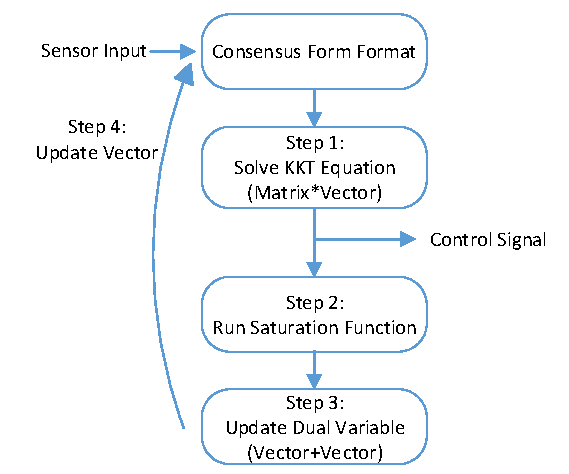
\includegraphics[scale=.75]{../figure/dataFlow.pdf}
%\DeclareGraphicsExtensions.
%\caption{MPC Control Dataflow using ADMM\label{fig:dataflow}}
%\end{figure}

The solution to\cref{eq:zi} is the result of a saturation function. The detailed processing steps are shown in Algorithm\cref{alg:ADMM}, which is pipelined in hardware. A common stopping criteria is to check if $\lVert \zeta^{i+1}-\zeta^i\rVert$ or $\lVert \upsilon^{i+1}-\upsilon^i\rVert$ is smaller than a certain value. We instead use a fixed number of iterations as the stopping criteria since for many control applications a relatively small number of iterations provides sufficient controller accuracy \cite{6422363}, and this reduces hardware complexity.

\begin{algorithm}
Start from $i=0$ with arbitrary $\zeta^0$ and $\upsilon^0$.
\SetKwRepeat{Do}{do}{until}
\caption{ADMM algorithm}\label{alg:ADMM}
\Do{stopping criterion is satisfied}{
$l:=
\begin{bmatrix}
	Q*R_k\\
	\textbf{0}
\end{bmatrix}-\rho (\zeta^{i}+\upsilon^{i})$   \tcp{Update Vector l}
	$\chi^{i+1}:=
	M_{11}*
	\begin{bmatrix}
	-l&x_{k}
	\end{bmatrix}^T$ \tcp{Solve KKT}
	$\zeta^{i+1}:=sat(\chi^{i+1}-\upsilon^i,\textbf{dom}\: {\mathcal{C}})$   \tcp{Saturation}
	$\upsilon^{i+1}:=\upsilon^i+\rho (\zeta^{i+1}-\chi^{i+1})$   \tcp{Update Dual}
	$i:=i+1$
}
\end{algorithm}

As a final note on Algorithm\cref{alg:ADMM}, the $\chi^{i+1}$ appearing in line 5 and 6 is substituted with $\alpha \chi^{i+1}+(1-\alpha )\zeta^{i}$.
%\begin{equation}
%\label{eq:re}
%\alpha x^{i+1}+(1-\alpha )z^{i}
%\end{equation}
$\alpha \in (0,2)$ is the relaxation parameter derived from Douglas-Rachford splitting. The convergence rate can be improved if $\alpha$ is properly selected. %For more details about relaxation parameter refer to\cite{Eckstein92onthe}.
\section{ADMM Hardware Architecture}\label{arch}
This section introduces the detailed hardware architecture to support Algorithm\cref{alg:ADMM}. Major focuses of the design were system parametrization, system scaling, and runtime reference trajectory setting. Finally, we analyze the computation latency and BRAM usage. The design is written in VHDL using Vivado 2015.4 IDE.
\subsection{ADMM Architecture Overview}
As shown in Fig.\cref{fig_arch}, the high-level hardware architecture is divided into Top and Bottom level for a modularized illustration. Top level is the Quadratic Programming Solver. It has a matrix-vector multiplier tree structure. Bottom level is composed of three parts: 1) Saturation Function (marked in green diagonal line), 2) Update Vector $\upsilon^i$ (marked in purple cross line), 3) Update Vector $l$ (marked in red). Some FIFOs which are used to store intermediate values are not shown in the figure. We use Block RAM(BRAM) to store the $\zeta^i$, $\upsilon^i$ vector and the boundary value box constraints $x$, $u$, and $\Delta u$.

\begin{figure}[t]
\centering
\captionsetup{justification=centering}
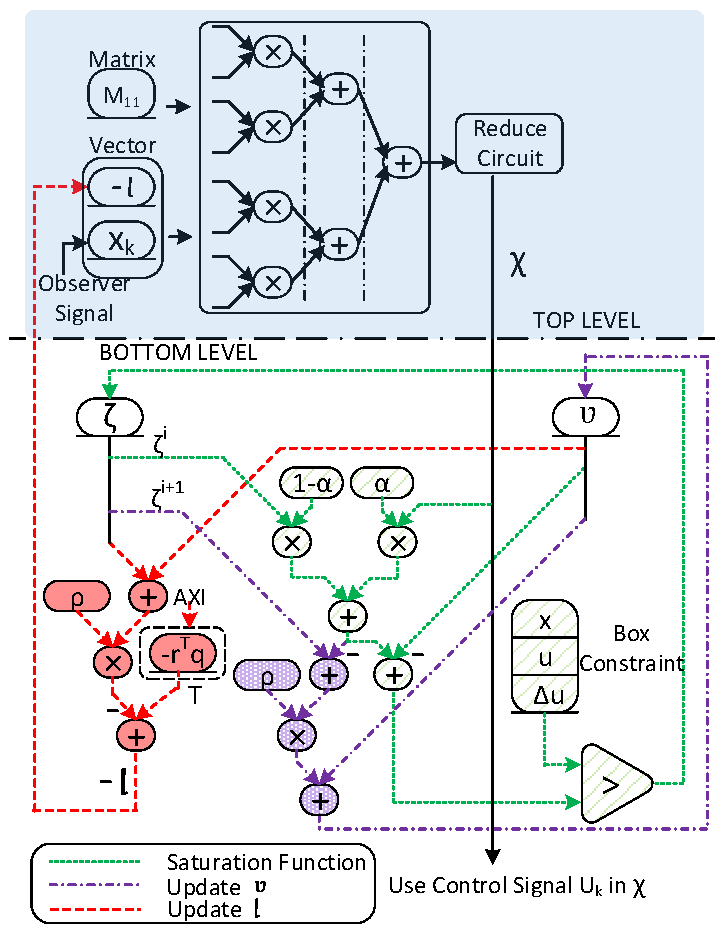
\includegraphics[scale=.59]{../figure/architecture.pdf}
\DeclareGraphicsExtensions.
\caption{Hardware Architecture for ADMM with Relaxation Parameter $\alpha$.\label{fig_arch}}
\end{figure}

We next describe the components of Fig.\cref{fig_arch} in greater detail:
\subsubsection{Matrix-vector Multiplier (MVM)}
The QP solver is similar to the architecture presented in\cite{Zhuo:2005:SMM:1046192.1046202} for parallelizing MVM of large sparse matrices. The MVM computation uses a tree structure. $D_p$ indicates the depth of the MVM tree. The total number of multipliers in the MVM tree is $2^{D_p}$ and the number of adders is $2^{D_p}-1$.

\subsubsection{Data Storage}
Block RAMs (BRAMs) are used as the primary on-chip memory of the MPC engine. We configure the BRAMs as true dual port, which provides two read and two write ports. Every multiplier in the MVM tree has a dedicated dual port BRAM attached, with one port feeding matrix data and one port feeding vector data.\par

According to the BRAM configuration datasheet, the BRAM has to be at least 36Kb. Since the matrix size is the square of the vector size, we reserve a small fraction of space for vector storage. Another solution is to use Look Up Tables (LUTs) to store the vector. In either case, the vector should be duplicated to avoid write back conflicts.\par
%18 Kb BRAM alone cannot be configured as true dual port BRAM. Thus each multiplier has to be attached with at least one 36 Kb BRAM, where only 32Kb memory is available when the data width is set as 32 bit. The system cascades 18Kb BRAM with the 36Kb BRAM to expand its storage. The number of 18Kb BRAM required for each multiplier is $\lceil max(N_E,1024)/512\rceil$. As we mentioned, $N_E$ is the number of matrix element we stored in the BRAM. The percentage of BRAM utilization in front of each multiplier is shown in Equation\cref{eq:uti}. Fig.\cref{fig_bram3} shows the BRAM unilization, which varies with $N_E$ in that BRAM. With this figure, we can easily know the utilization of BRAMs after we compute the number of matrix element inside. Generally with more and more matrix data stored in the BRAM, the utilization will increase.
%
%\begin{equation}
%\label{eq:uti}
%Utilization=\frac{N_E}{\lceil \frac{max(N_E,1024)}{512}\rceil *512}
%\end{equation}
%
%\begin{figure}[!ht]
%\centering
%\captionsetup{justification=centering}
%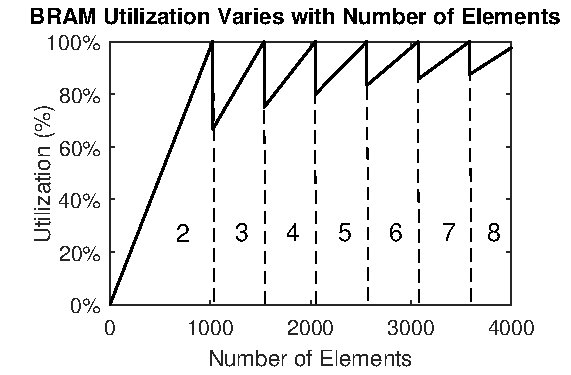
\includegraphics[scale=.78]{../figure/BRAM3.pdf}
%\DeclareGraphicsExtensions.
%\caption{The utilization of BRAMs varies with number of elements stored regarding each multiplier. The digital number between dash line and solid line is the number of 18Kb BRAM attached in front of each multiplier.\label{fig_bram3}}
%\end{figure}

We use $N_{BRAM}$ to represent the number of available 36Kb BRAMs. $N_{DSP}$ is the number of DSP slices on-chip. If the hardware resources meet inequality condition\cref{eq:com}, the BRAM will hinder the scalability of the system without the support of the reduce circuit. This conclusion is based on the assumptions that 1) each multiplier and adder consume one DSP slice; 2) each MVM multiplier requires at least one 36kb BRAM.
According to the Zynq datasheet, only the Z-7100 device from the Zynq-7000 family is unconformable to the inequality condition\cref{eq:com}, which indicates that the on-chip memory is the resource bottleneck for most of the Zynq-7000 family.
\begin{equation}
\label{eq:com}
2*N_{BRAM}\geq N_{DSP}\geq 63.25\sqrt{N_{BRAM}}
\end{equation}

%\subsection{Potential Computation Parallism Estimation}
%\label{aaa}
%The computation can be further paralleled by introducing multiple processing units (PUs) as is shown in Fig.\cref{fig_hp}. Each PU has its own ADMM component like in Fig.\cref{fig_arch}. 
%The $M_{11}$ matrix is separated row by row. We store each row from PU\big[1\big] to PU\big[K\big] and start over until the whole matrix is stored into PU BRAMs. In this way, we can avoid conflict of writing vector back if their destination is the same BRAM. After the data fills the processing pipeline, $K$ new vector elements will come out of the pipeline during the same clock cycle. Since these elements are stored in different BRAMs, the write-back operation can be done in one clock cycle. We call this mechanism duplication.
%
%\begin{figure}[!ht]
%\centering
%\captionsetup{justification=centering}
%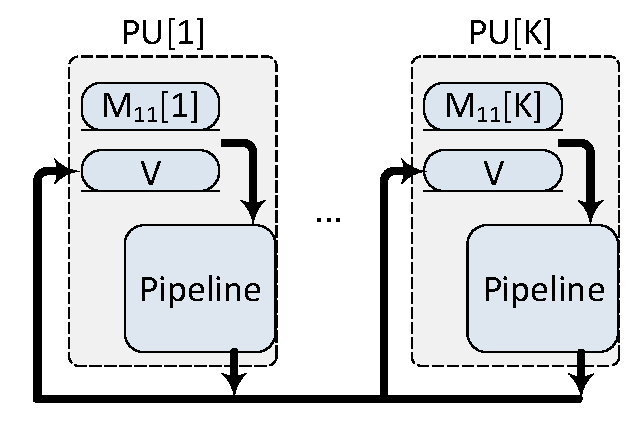
\includegraphics[scale=.40]{../figure/highParallel.pdf}
%\DeclareGraphicsExtensions.
%\caption{Highly paralleled ADMM Hardware Solution\label{fig_hp}}
%\end{figure}
%
%The latency shares the same formula as Equation.\cref{eq:tl} except for the $L_{read\_ M_{11}}$ term. The $L_{read\_ M_{11}}$ is inverse proportional to parallelism $K$ in Equation.\cref{eq:klemr} .
%\begin{equation}
%\label{eq:klemr}
%L_{read\_ M_{11}}=\frac{N_{ROW}}{K}*(N_R+1)
%\end{equation}

\subsubsection{Reduce Circuit}

The purpose of the reduce circuit is to let us balance between resource usage and the number of MVM pipeline stages. Fig.\cref{fig_red} shows a reduce circuit structure, which is cascading two smaller reduce circuits.\par
\begin{figure}[t]
\centering
\captionsetup{justification=centering}
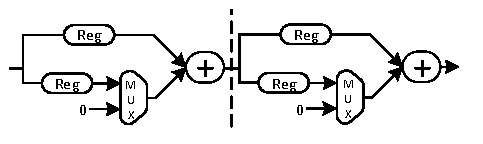
\includegraphics[scale=0.9]{../figure/Reduce.pdf}
\DeclareGraphicsExtensions.
\caption{Reduce Circuit Architecture with Two Cascaded Adders\label{fig_red}}
\end{figure}
The reduce circuit allows a single row of the matrix and vector to be separated into segments, and each segment is fed into the MVM pipeline in consecutive clock cycles. The reduce circuit accumulates the sum of each segment and generates a final result out of the last reduce stage. By employing more cascading levels, we can divide each row of the matrix into smaller segments at the cost of increasing latency due to increased pipeline stages at the reduce circuit. Suppose the depth of the MVM tree is $D_p$, and the number of $M_{11}$ rows is $N_{ROW}$ and columns is $N_{COL}$. Then the number of adders in the reduce circuit that our system requires is $N_R=\lceil N_{COL}/2^{D_p}\rceil-1$. The number of clock cycles to merge all the matrix and vector data into the MVM pipeline is:
\begin{equation}
\label{eq:md}
L_{read\_ M_{11}}=N_{ROW}*(N_R+1)
\end{equation}

\subsubsection{Saturation Function}
Fig.\cref{fig_arch} contains the hardware for saturation function. We assume each variable has same absolute upper and lower boundary value so that we just store the positive boundary values in the box constraint BRAM. The result of $\chi^{i+1}-\upsilon^{i}$ is compared with the box constraints. If the absolute value of $\chi^{i+1}-\upsilon^{i}$ is smaller than the box constraint, we output the value directly. Else, if the value is larger, we output the box constraint using the sign of $\chi^{i+1}-\upsilon^{i}$.

\subsection{Trajectory Setting During Runtime}
\begin{figure}[t]
\centering
\captionsetup{justification=centering}
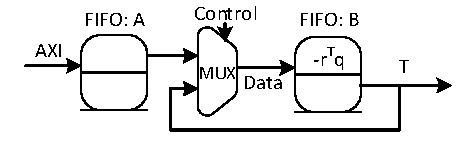
\includegraphics[scale=.75]{../figure/trajectoryProfile.pdf}
\DeclareGraphicsExtensions.
\caption{Runtime Trajectory Planning\label{fig_traj}}
\end{figure}

MPC can optimize a system's following of a trajectory multiple time steps ahead so that system can react accordingly in advance. Our controller can set the desired trajectory during runtime. For example, we may want to update a UAV's flight path while it is in the air.\par

We use two FIFOs to realize the functionality. The architecture is shown in Fig.\cref{fig_traj}, which is located in the dashed square marked by 'T' in Fig.\cref{fig_arch}. First, we configure FIFO:A and FIFO:B. FIFO:B stores the trajectory data for the current computation, and FIFO:A stores the future trajectory data. When computing the $l$ vector, we read FIFO:B, use the data and write its output back to itself, which will be used for next converge iteration. In the last iteration, we discard the front $N$ numbers after reading, and write the remaining back to FIFO:B. Next, we load $N$ new trajectory data from FIFO:A into FIFO:B. In this way, each trajectory data shifts forward one sample step, and we fill the last trajectory point with a new one. Since writing to FIFO:A is independent of operations on FIFO:B, we can write new state trajectory data to FIFO:A at any time before FIFO:B goes empty.

\subsection{Latency Analysis}

Table\cref{tab:lat} gives computation latency. The floating point multiplier latency is $L_M$=8; the floating point adder latency is $L_A$=11, the comparator latency is $L_C$=2. We call $L_{bt}+L_{bl}$ pure processing stages, namely the number of pipeline stages from an element entering the MVM pipeline to finishing.

\begin{center}
\captionof{table}{Computation Latency}
\label{tab:lat}
\begin{tabular}{ c|c } 
 \hline
 Binary Tree ($L_{bt}$)& $L_M+D_pL_A+N_R(L_A+2)$\\ 
\hline
 Bottom Level ($L_{bl}$)& $6L_A+3L_M+L_C$\\ 
 \hline
\end{tabular}
\end{center}

%To be noticed here, the result can only be written back into BRAM after all the matrix and vector data have been merged into the MVM pipeline since the two ports of each BRAM are being used as reading ports (one for the matrix $M_{11}$, one for the vector $V$) during the time. Assuming the data is blocked for $L_f$ pipeline stages in the form of walking through the FIFO in the lower-left portion of Fig.\cref{fig_arch} before writing back, then $L_f$ is computed as in Equation\cref{eq:lf}. 
%\begin{equation}
%\label{eq:lf}
%L_{f}=max\Big(0,L_{mer}-(L_{bt}+L_{bl})\Big)
%\end{equation}
%
%The total clock cycle for doing one iteration of Algorithm\cref{alg:ADMM} is:
%\begin{align*}
%L_{ADMM}&=L_f+L_{bt}+L_{bl}+L_{mer}\\
%&=max\Big(2*L_{mer},L_{mer}+L_{bt}+L_{bl}\Big)
%\numberthis \label{eq:tl}
%\end{align*}
%
%From Formula\cref{eq:tl} we see that if $L_{mer}$ is greater than $L_{bt}+L_{bl}$, the total pipeline stages is irrelative to the pure processing stages. This finding means that even though fixed-point adder/multiplier takes one single clock cycle to get to the result, for a large matrix, the pipeline stages in Figure.\cref{fig_arch} has no effect on your total processing time $L_{ADMM}$, which proves that floating-point is as fast as fixed-point arithmetic in this situation. 

The total latency $L_{ADMM}$ is shown in Equation.\cref{eq:tl}, which is the sum of pure processing stages and the clock cycles to finish fetching all the matrix and vector data into MVM tree ($L_{read\_ M_{11}}$). 
\begin{equation}
\label{eq:tl}
L_{ADMM}=L_{bt}+L_{bl}+L_{read\_ M_{11}}
\end{equation}

The architecture by default fetches one row per clock cycle or we can break each row into several pieces and accumulate each piece through the reduce circuit. However, under most cases, $N_{COL}/2^{D_p}$ is not an integer, thus some BRAMs store '0's to pad the final piece of the matrix row. These padding '0's occupy BRAM space and decrease the scalability of the design. The problem can be solved via introducing a simple state machine that tells the hardware which DSP should be fed '0' instead of reading data from BRAM.

%\subsection{Potential Computation Parallism Estimation}
%\label{PCPE}
%The computation can be further paralleled by introducing multiple processing units (PUs) as is shown in Fig.\cref{fig_hp}. Each PU has its own ADMM component like in Fig.\cref{fig_arch}. 
%%The reduce circuit is no more recommended in this scenario since the on-chip resource is not considered as a limitation. 
%The $M_{11}$ matrix is separated row by row. We store each row from PU\big[1\big] to PU\big[K\big] and start over until the whole matrix is stored into PU BRAMs. In this way, we can avoid conflict of writing vector back if their destination is the same BRAM. After the data fills the processing pipeline, $K$ new vector elements will come out of the pipeline during the same clock cycle. Since these elements are stored in different BRAMs, the write-back operation can be done in one clock cycle. We call this mechanism duplication.
%
%\begin{figure}[!ht]
%\centering
%\captionsetup{justification=centering}
%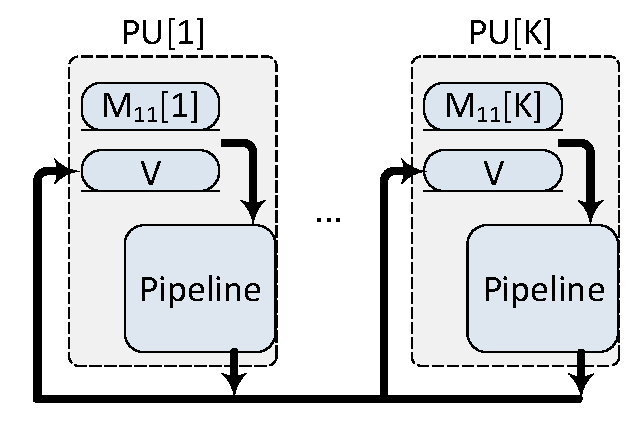
\includegraphics[scale=.55]{../figure/highParallel.pdf}
%\DeclareGraphicsExtensions.
%\caption{Highly paralleled ADMM Hardware Solution\label{fig_hp}}
%\end{figure}
%
%The latency shares the same formula as Equation.\cref{eq:tl} except for the $L_{read\_ M_{11}}$ term. The $L_{read\_ M_{11}}$ is inverse proportional to parallelism $K$ in Equation.\cref{eq:klemr} .
%\begin{equation}
%\label{eq:klemr}
%L_{read\_ M_{11}}=\frac{N_{ROW}}{K}*(N_R+1)
%\end{equation}


\section{Evaluation}\label{eva}
This section describes our SW/HW co-design evaluation methodology. We evaluate our design using a Plant-on-Chip (PoC), which emulates the physical behavior of a linear system~\cite{VyaKum13A}. We provide post place\&route results including resource usage and maximum clock frequency. We then compare our work with other related works.
\subsection{Mass-spring System}
The system we use to test our controller is a mass-spring model, which is considered as a benchmark in \cite{6927473}, \cite{Jerez:2011:FIS:1950413.1950454} and many recent works use it to validate their hardware controller. The physical system is illustrated in Fig.~\ref{fig_ms}. The objective is moving masses to desired positions by applying a force to each mass. The state vector consists of the position ($P$) and speed ($\dot P$) of each mass\footnote{$P$ is the position relative to the initial position}. The state space model size increases quadratically as the number of masses increases. We constrain the position of each mass within 0.5m to avoid collision between adjacent masses. Each mass is 1Kg, and the spring constant is 1N/m. The input force ($U$) is limited to $\pm 0.5N$ and the change of input force between each sample period (i.e. rate of change, $\Delta U$) is 0.1N, as in \cite{jerez2014embedded}. The sample period is 0.1s. The prediction horizon ($H_p$) and input horizon ($H_u$) are both 12. The cost constant for position $P$, input force $U$ and input-rate $\Delta U$ are 80, 1 and 0 (we are not trying to minimize $\Delta U$ during the control process) respectively.

\begin{figure}[t]
\centering
\captionsetup{justification=centering}
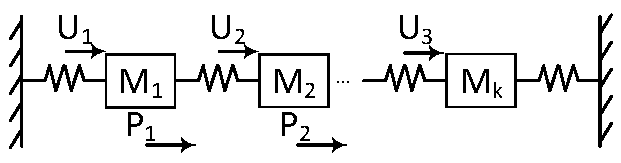
\includegraphics[scale=.48]{../figure/massspring.pdf}
\DeclareGraphicsExtensions.
\caption{Mass-spring System\label{fig_ms}}
\end{figure}

\subsection{Plant on Chip Emulation}
We conducted our experiments on a Zynq-7020 device. A Plant-on-Chip (PoC) was deployed onto the FPGA's Programable Logic (PL) fabric to emulate the mass-spring system shown in Fig.~\ref{fig_ms}. The PoC executes state space Equations~\ref{eq:xk} and~\ref{eq:yk} with input $u_k$ received from a hardware or software-based controller. The state of the PoC and control commands are logged out of band, using a UART interface, which is convenient for plotting the controller behavior at runtime.\par
The MPC controller requires the CPU to configure the co-processor BRAM content with the matrix $M_{11}$. When running the MPC hardware controller at 100 MHz, it computes $u_k$ in 347.8$\mu s$ using a $D_p$=3 MVM tree and executes 20 fixed converge iterations.\par
The hardware control graph is shown in Fig.~\ref{fig_mp}. The red dashed line is the software configured trajectory, and the blue line is the actual mass position. The first 100 points of the trajectory are stored in the trajectory FIFO during configuration, which reflects 0s$-$10s of red trajectory line. The remainder of the trajectory is configured during runtime. The input force and the input force rate of change are shown in Fig.~\ref{fig_mu}. From the graph, we can see that the control signal and control signal rate of change respect their bounding constraints of $\pm$0.5N and $\pm$0.1N per time step respectively.

\begin{figure}[t]
\centering
\captionsetup{justification=centering}
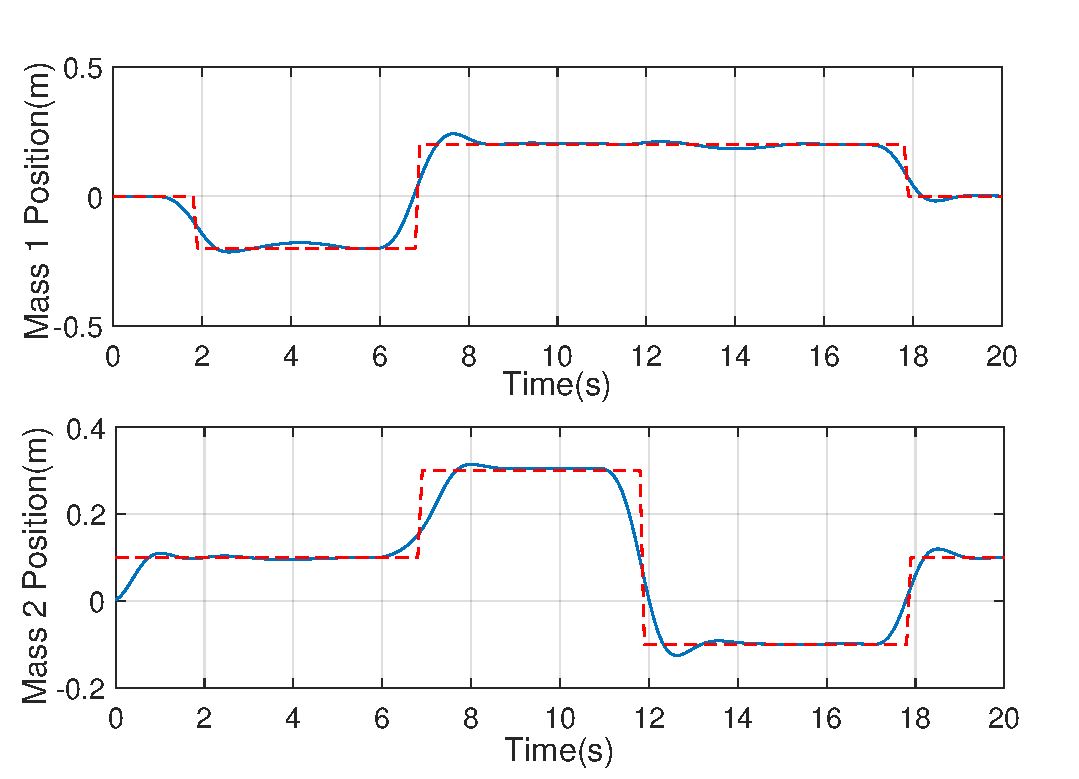
\includegraphics[scale=.45]{../figure/MP.pdf}
\DeclareGraphicsExtensions.
\caption{Mass Position Change with respect to Planned Trajectory. Red dashed line is the planned trajectory, and the blue line is the actual trajectory.\label{fig_mp}}
\end{figure}

\begin{figure}[t]
\centering
\captionsetup{justification=centering}
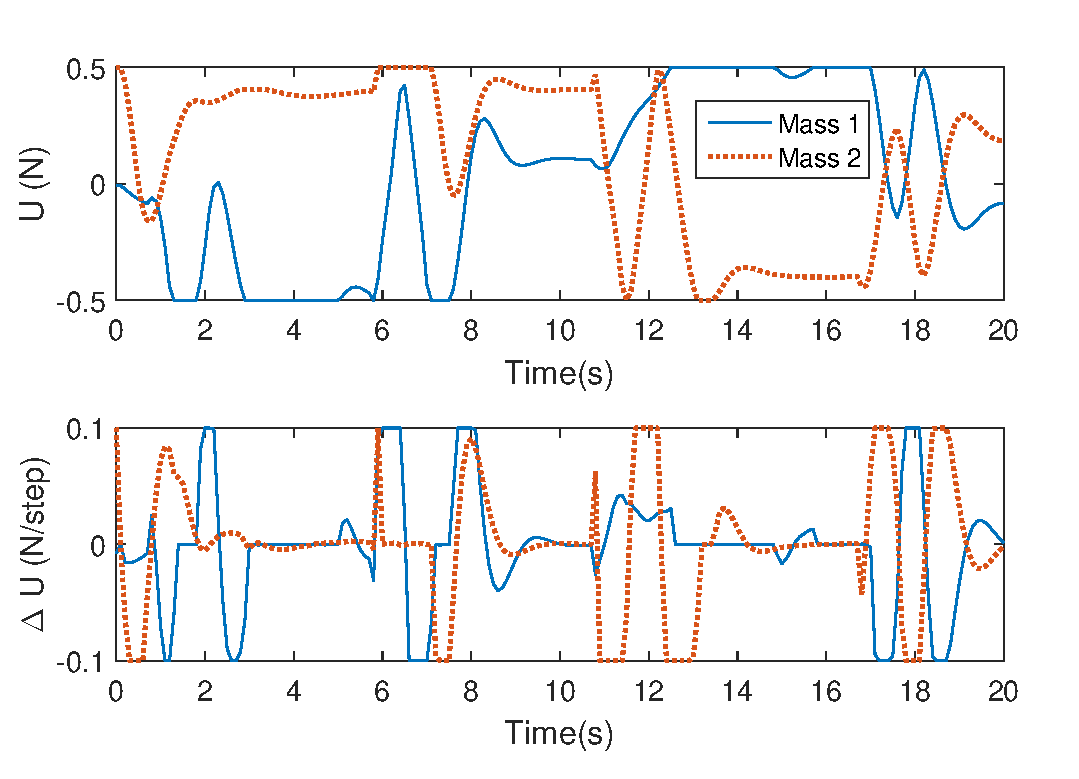
\includegraphics[scale=.45]{../figure/MU.pdf}
\DeclareGraphicsExtensions.
\caption{Control Signal $U$ and $\Delta U$. Blue line is the input force and the force rate of change for $M_1$, red dashed line is for $M_2$.\label{fig_mu}}
\end{figure}

\subsection{SW/HW Co-design}
The on-chip ARM processor transfers a pre-generated $M_{11}$ matrix into the reconfigurable fabric's BRAMs through the AXI bus. Additionally, the on-chip ARM processor can access memory-mapped registers resident in the reconfigurable fabric to indicate when the MPC hardware engine should start and stop, and for updating the desired trajectory at runtime.
The system block design is shown in Fig.~\ref{fig_copro}. The design steps are:
\begin{enumerate}
\item According to system requirements, generate the bitstream in Vivado, and $M_{11}$ matrix in Matlab.
\item Store $M_{11}$ to BRAM via AXI bus using ARM software.
\item ARM software configures trajectory and box constraints.
\item Send start signal to the PoC, and collect data through UART to external computer and plot graph.
\end{enumerate}\par
As we can see from the design steps, a control engineer can easily handle each step. In addition, when we apply the hardware control to another system with different parameters and size, the design can be easily adjusted.
% For the control interface design example between FPGA and physical plant, refer to\cite{telba2015dc}.

\begin{figure}[t]
\centering
\captionsetup{justification=centering}
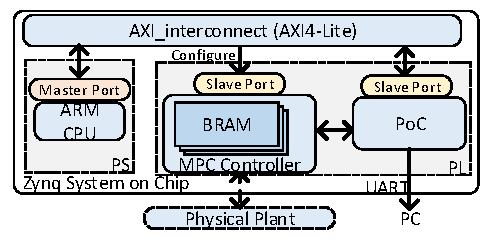
\includegraphics[scale=.84]{../figure/copro.pdf}
\DeclareGraphicsExtensions.
\caption{Top Level System Overview\label{fig_copro}}
\end{figure}


\begin{figure}[t]
\centering
\captionsetup{justification=centering}
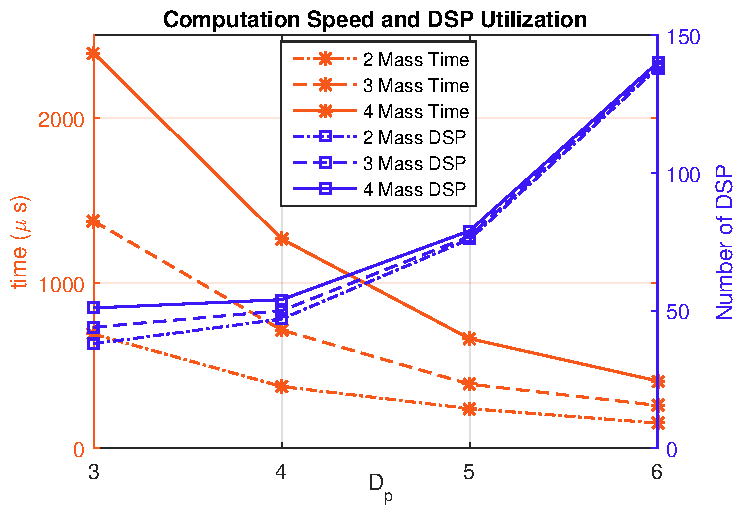
\includegraphics[scale=.65]{../figure/dsp.pdf}
\DeclareGraphicsExtensions.
\caption{Computation time of 40 converge iteration loops and DSP usage for different system configurations from simulation. Computation time is marked by $\ast$, number of DSPs is marked by $\Box$. Hardware speed is 100MHz.\label{fig_ct}}
\end{figure}

\subsection{Computation Speed Versus Hardware Resources}
The relationship between DSP usage, $D_p$, and system size is shown in Fig.\cref{fig_ct}. As $D_p$ increases, the size of the reduce circuit will decrease thus reducing computation time. The DSP resources used is modifiable. The more DSPs we use, the faster computation speed we achieve. Consider a situation where an FPGA has few DSP resources available, our proposed architecture can still execute the controller by decreasing the MVM depth, at the cost of increased computing time.\par

\subsection{Resource Utilization and Timing Summary}
Table~\ref{tab_hrs} shows the resource utilization of the ADMM architecture. Each floating-point multiplier and adder use one DSP48E. We used the maximum number of pipeline stages supported by the Xilinx floating point adder(11) and multiplier(8) IP cores. Each memory attached to the MVM multiplier tree is composed of 2 36Kb BRAMs. BRAMs are also used for FIFOs in the MVM tree and Bottom level. The Zynq-7020 can hold an MVM tree having a depth up to 6. Generally, the clock frequency can easily reach 100MHz. 
\begin{table}[!ht]
\centering
\captionsetup{justification=centering}
\caption{Zynq-7020 Hardware Resource Usage}\label{tab_hrs}
\begin{tabular}{ >{\centering\arraybackslash} m{0.6cm} |>{\centering\arraybackslash} m{0.9cm}|>{\centering\arraybackslash} m{0.9cm}|>{\centering\arraybackslash} m{0.9cm}|>{\centering\arraybackslash} m{0.85cm}|>{\centering\arraybackslash} m{1cm} }

\hline
\multicolumn{1}{c|}{MVM}&\multicolumn{1}{c|}{Flip-Flops}&\multicolumn{1}{c|}{LUTs}&\multicolumn{1}{c|}{18Kb }&\multicolumn{1}{c|}{DSP48E}&\multicolumn{1}{c}{Maximum }\\

Size $D_p$ &(106400 total)&(53200 total)&BRAM (280 total)&(220 total)&Frequency \\ 
 
\hline

3&18147&12746&55&38&151.149MHz\\
\hline 
4& 21058 & 15103&87&47&144.885MHz\\
\hline 
5& 32425 & 23391 &151&76&143.699MHz\\
\hline 
6& 57167 & 41273&279&138&133.298MHz\\
\hline

\end{tabular}
\end{table}

We also tested the resource scaling on a Zynq Ultrascale. It can reach 340MHz when deploying a $D_p=8$ MVM tree.

%\subsection{Single Precision Floating Point Error}
%We compare the single precision floating point with double precision floating point by running the mass spring system with ADMM iteration ranging from 10 to 40. The error is shown in Table.~\ref{tab_pe}. We also show the error between 20 bit fraction fixed point and double precison floating point.
%
%\begin{table}[!ht]
%\centering
%\captionsetup{justification=centering}
%\caption{Percentage of Error using FLoating Point and Fixed Point(20 bit fraction per iteration. $I$ means the total number of iterations) in each iteration.}\label{tab_pe}
%\begin{tabular}{ >{\centering\arraybackslash} m{0.6cm} |>{\centering\arraybackslash} m{0.6cm}|>{\centering\arraybackslash} m{0.6cm}|>{\centering\arraybackslash} m{0.6cm}|>{\centering\arraybackslash} m{0.6cm}|>{\centering\arraybackslash} m{0.6cm}| >{\centering\arraybackslash} m{0.6cm}| >{\centering\arraybackslash} m{0.6cm} }
%
%\hline
%\multicolumn{1}{c|}{Type $\backslash$ I}&\multicolumn{1}{c|}{10}&\multicolumn{1}{c|}{15}&\multicolumn{1}{c|}{20 }&\multicolumn{1}{c|}{25}&\multicolumn{1}{c|}{30}&\multicolumn{1}{c|}{35}&\multicolumn{1}{c}{40}\\
%\hline
%SP&7.3&1.8&2.4&1.7&1.3&0.75&0.12\\
%Floating&e-6&e-6&e-6&e-6&e-6&e-6&e-6\\
%\hline 
%Fixed& 0.58 & 0.49 & 0.42 & 0.37 & 0.32 & 0.28 & 0.25\\
%\hline
%\end{tabular}
%\end{table}
%
%We find that floating point error is much smaller than 20 fractional fixed point. Thus we run our experiment only use 20 iterations.

\subsection{Comparision with other Works}
Table~\ref{tab_cmp} provides a comparative summary of our work with two other FPGA accelerated MPC works and a software implementation. For the hardware work, one is IPM based \cite{6927473}, and another is ADMM based \cite{jerez2014embedded}, like ours. Starting with the IPM based work, it can be seen when compared against the ADMM-based approaches using about half the number of multipliers (\textasciitilde{200}) for about the same number of decision variables (\textasciitilde{200}) our approach is about 50x faster (2,650us vs. 46.1us) than the IPM implementation and the other ADMM work \cite{jerez2014embedded} is about 100x faster (2,650us vs. 23.4us). As explained in Section~\ref{rw}, this is due to the ADMM algorithm requiring less computation per convergence iteration. The software implementation, \cite{6422363}, is ADMM based, and is run on a 3.4GHz Xeon processor. We estimate for 262 variables that this SW solution would take 850 $\mu s$ if the average number of iteration maintains in 35.1.\par
 \begin{table*}[!ht]
\small
\centering
\captionsetup{justification=centering}
\caption[Caption for LOF]{Hardware Computation Time per Iteration between Related Work.\label{tab_cmp}\protect\footnotemark}
%\caption{Hardware Computation Time per Iteration between Related Work.\label{tab_cmp}}

\begin{tabular}{|*{9}{c|}}\hline

&\makebox[2.2em]{Method}&\makebox[4em]{Data Format}&\makebox[4em]{Chip Series}&\makebox[2.5em]{$f_{clk}$}&\makebox[4em]{\#Multipliers}&\makebox[2.5em]{Iteration}&\makebox[3em]{\#Opt Var}&\makebox[6em]{Running Time}\\
\hline
\hline

\multirow{5}{*}{This Paper} &\multirow{5}{*}{ADMM}&\multirow{5}{*}{floating-point}&\multirow{3}{*}{Zynq-7020}&\multirow{3}{*}{130MHz}&\multirow{2}{*}{72 ($D_p$=6, K=1)}&\multirow{5}{*}{40}&\multirow{1}{*}{204}&\multirow{1}{*}{314.2 $\mu s$}\\
\hhline{~~~~~~~--}
&&&\multirow{0}{*}{}&&&&350*&{717.2 $\mu s$}\\
\hhline{~~~~~-~--} 
&&&\multirow{1}{*}{}&&80 ($D_p$=5, K=2)&&\multirow{3}{*}{204}&{291.4 $\mu s$}\\
\hhline{~~~---~~-}
&&&\multirow{1}{*}ZU9EG&\multirow{2}{*}{340MHz}&264 ($D_p$=8, K=1)&&&{46.1 $\mu s$}\\
\hhline{~~~~~-~~-}
&&&\multirow{1}{*}(Zynq UltraScale+)&&792 ($D_p$=8, K=3)&&&{30.1 $\mu s$}\\ 
\hline
\hline

\multirow{2}{*}{HW\cite{jerez2014embedded}} &\multirow{2}{*}{ADMM}&\multirow{2}{*}{fixed-point}&Virtex-6 (LX75)&\multirow{2}{*}{400MHz}&\multirow{1}{*}{216 (K=1)}&\multirow{2}{*}{40}&\multirow{2}{*}{216}&\multirow{1}{*}{23.4$\mu s$}\\ 
\hhline{*4~|*1~|*4~}
%&&&LX75&& &&&\\
\hhline{*3~|-|~|-|*2~|-}
\multirow{1}{*}{} &\multirow{1}{*}{}&\multirow{1}{*}{}&Virtex-6 (SX475)&\multirow{0}{*}{}&\multirow{1}{*}{1512 (K=7)}&\multirow{1}{*}{}&\multirow{1}{*}{}&\multirow{1}{*}{4.90$\mu s$}\\ 
\hhline{*4~|*1~|*4~}
%&&&SX475&& &&&\\
\hline
\hline

\multirow{1}{*}{HW\cite{6927473}} &\multirow{1}{*}{IPM}&\multirow{1}{*}{floating-point}&Virtex-7 (XC7VX485T)&\multirow{1}{*}{200MHz}&\multirow{1}{*}{448}&\multirow{1}{*}{10}&\multirow{1}{*}{240}&\multirow{1}{*}{2,650 $\mu s$}\\ 
\hhline{*9~}
%&&&(XC7VX485T)&&&&&\\
\hline
\hline

\multirow{1}{*}{SW\cite{6422363}} &\multirow{1}{*}{ADMM}&\multirow{1}{*}{floating-point}& Quad-core Intel
Xeon&\multirow{1}{*}{3.4GHz}&\multirow{1}{*}{n/a}&\multirow{1}{*}{35.1}&\multirow{1}{*}{525}&\multirow{1}{*}{3,400 $\mu s$}\\ 
\hhline{*9~}

\hline
\end{tabular}
\end{table*}

When comparing our approach with the ADMM based approach of \cite{jerez2014embedded}, for about 200 multipliers and 200 decision variables, it can be seen that our approach is about two times slower (i.e. 46.1 us vs. 23.4 us). The primary reason for this is that in \cite{jerez2014embedded} fixed point arithmetic is used, while our implementation uses 32-bit floating point arithmetic. The main way in which this impacts performance is that the floating point adders required 11 pipelining stages to maximize clock frequency, while fixed point addition can be done at a high clock rate in one clock cycle. For the size of matrices being operated on (limited by on-chip memory), the number of adder pipeline cycles to fill the processing pipeline (\textasciitilde{88} for an MVM tree of depth 8) is nearly half the number of matrix rows (\textasciitilde{200}) read into the MVM tree. This accounts for a vast majority of the two times difference in performance. However, for this cost in performance, we gain the convince of software and control algorithm developers not having to deal with the complexities of working with custom fixed-point number formats, easing the process of deploying a designed controller into our MPC accelerator. For physical systems requiring sub-millisecond controller updates rates, this is a good tradeoff, however for controllers requiring 10’s of microsecond updates rates using a fixed-point approach is more appropriate with today’s FPGA capabilities. The important question to answer is for your application is the convenience of using floating point worth the performance tradeoff.
 
The Reduce circuitry implemented in our architecture naturally allows our design to scale to large numbers of decision variables using a nearly arbitrarily small number of multipliers at the cost of speed, as is illustrated in the 350* entry of Table~\ref{tab_cmp}, while \cite{jerez2014embedded} does not have such a mechanism for scaling the number of decision variables above the number of multipliers in the system. This gives our MPC engine the flexibility to be deployed into System-on-Chip FPGA applications that may not have many multipliers to allocate to an MPC computation engine. Two ADMM tuning features implemented in our ADMM architecture that is not implemented by \cite{jerez2014embedded} is a relaxation parameter ($\alpha$) and a dual update step length ($\rho$), which can be used to tune the convergence rate of ADMM for a given system.

A final point of comparison is that this work tightly integrates an on-chip ARM processor with the MPC compute engine. This provides Controls or Software engineers a convenient software mechanism for configuring the controller for arbitrary systems, updating the desired trajectory of the system at runtime, and tuning the ADMM $\alpha$ and $\rho$ parameters.


\footnotetext{K indicates the number of times the core MPC engine with $D_p$ MVM tree is duplicated to process Matrix rows in parallel}


\section{Conclusion}\label{con}
We have presented an MPC acceleration engine that is tightly coupled to an ARM processor embedded on the same chip. Our acceleration engine has been designed to allow trading off between performance and hardware resource usage. Our tight interface with an on-chip ARM processor allows software to easily update the configuration of the acceleration engine to control a wide range of systems, and to adjust the desired system trajectory at run-time. An avenue of future work is examining the architectural details required for interfacing and managing external sensors to extend our evaluation from controlling a real-time Plant on Chip to actual physical systems, such as quadcopters.
\bibliographystyle{IEEEtran}
\bibliography{MPC}



% that's all folks
\end{document}


